\documentclass[a4paper,10pt]{report}
\usepackage[T1]{fontenc}
\usepackage{framed}
\usepackage{lmodern}
\usepackage{textcomp}
\usepackage{graphicx}
\usepackage[utf8x]{inputenc}
\usepackage[italian, english]{babel}
\usepackage{geometry,setspace,listings,graphicx,lettrine,float,hyperref,eurosym,fancyhdr,booktabs,bookmark,titling}
\usepackage[dvipsnames]{xcolor}
\usepackage{listings}
\lstset{
  language=bash,
  basicstyle=\ttfamily
}
\graphicspath{ {../images/} }

\renewcommand*\footnoterule{}
\geometry{a4paper,top=3cm,bottom=3cm,left=3cm,right=2.5cm}
\singlespacing

\fancypagestyle{plain}
{
	\fancyhf{}
	\rfoot{\thepage}
}
\pagestyle{fancy}
{
	\fancyhf{}
	\headsep=40pt
	\lhead{\slshape \rightmark}
	\rhead{\slshape \leftmark}
	\rfoot{\thepage}
}
\begin{document}
  \thispagestyle{empty}
  \enlargethispage{60mm}
  \begin{center}
    \Large{\textsc{Università degli studi di Napoli Parthenope}}\\
    \large{Corso di laurea in Informatica}\\
    \large{Dipartimento di Scienze e Tecnologie}\\
    \vspace{25mm}
    \textbf{\Huge{\textsc{Bitcoin}}}\\
    \Large{Progetto d'esame Reti dei Calcolatori}\\
    \vspace{7mm}
    \begin{figure}[h]
    	\begin{center}
    	   
\includegraphics[scale=0.2]{parthenope.jpeg}
      \end{center}
    \end{figure}
    \vspace{35mm}
    \textbf{Vittorio FONES 0124001384}
    \vspace{5mm}

    \large{A. A. 20018-2019}
  \end{center}

  \pagenumbering{Roman}


  \tableofcontents
  \listoffigures

  \chapter{Descrizione del progetto}
  \pagenumbering{arabic}
	\lettrine[lraise=0.1]{C }on il seguente elaborato si intende illustrare il lavoro svolto per la realizzazione del progetto Bitcoin, il cui scopo è quello di creare una rete peer to peer usata per la gestione di una blockchain e l'utilizzo della stessa. Il progetto è stato sviluppato nel linguaggio C, attenendosi allo standard Posix come illustrato durante il corso e sul libro GAPIL: per l'appunto il software gira anche sotto piattaforma Mac OS, oltre che su distribuzioni Linux quali Debian e Arch Linux. \newline \newline Di seguito viene allegata l'introduzione della traccia sviluppata: \begin{framed} Si vuole realizzare un sistema per la gestione di una criptovaluta basato su una rete P2P. Il sistema è basato sulla gestione di una blockchain, ovvero una sequenza di blocchi in cui ogni blocco contiene una transazione. Il sistema si compone di due tipi di nodi: NodiN e NodiW. I NodiN creano la rete P2P e gestiscono la blockchain. Inoltre stampano la blockchain ogni volta che viene aggiunto un blocco: (blocco 1)-> (blocco 2)-> (blocco 3)-> (blocco 4). I NodiW gestiscono i wallet (portafogli virtuali) che consentono di inviare e ricevere pagamenti. Ad ogni nuovo pagamento inviato o ricevuto il nodo stampa la transazione ed il totale del portafogli. \end{framed}
	Per evitare qualunque tipo di problema d'ora in avanti i nodi\_w verranno chiamati semplicemente wallet.

  \chapter{Descrizione e schemi dell'architettura}
	Per creare la rete si è deciso di non adottare entità esterne, che seppure fossero venute in aiuto per l'automatizzazione della stessa rete, avrebbe reso il concetto di cryptovaluta meno reale, andando a rendere semi-centralizzata o peggio la rete peer to peer. Nonostante ciò si è cercato di non andare oltre la traccia, per cui tutti i casi reali quali il mining, la cifratura, creazione di hash e validificazione dei blocchi e altro, non sono stati presi in cosiderazione.\newline
	La rete peer to peer è composta dai nodi\_n che nel loro insieme formano una rete decentralizzata. Ogni nodo ha un pannello di controllo in cui è possibile interfacciarsi con altri nodi e vedere lo stato delle proprie attività, tra cui la blockchain al momento. A questi verranno poi connessi i nodi\_n: una volta collegato ad un nodo\_n, un wallet potrà effettuare movimenti di BitCoin, sarà poi il nodo\_n che provvederà a creare il blocco e diffonderlo.

  \begin{figure}[H]
  \center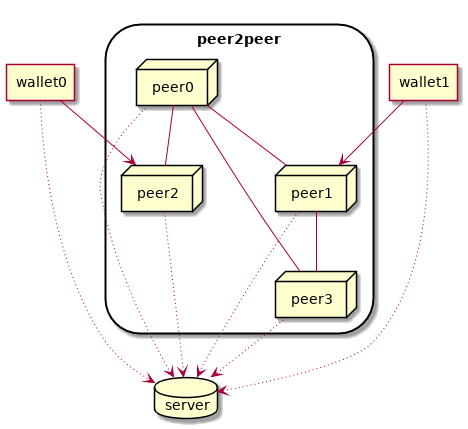
\includegraphics[scale=0.50]{arch.png}
  \caption{Architettura di sistema.}
  \end{figure}

  \chapter{Descrizione e schemi del protocollo applicazione}
  Di seguito sono riportati gli schemi dei principali protocolli applicazione.
  \section{Primo aggancio, scarico blockchain e flooding}
Per capire meglio lo scenario mostrato in figura, definiamo un Nodo\_0 e un Nodo\_N. Al Nodo\_N viene fatta richiesta di aggancio da parte del Nodo\_0, connesso a sua volta con più nodi e un wallet.\newline Inviando un tipo definito da programma, \textbf{request\_t}, il Nodo\_0 richiede al Nodo\_N di entrare a far parte della rete. Avvenuta la connessione bisognerà sincronizzare la blockchain, inviandosi i blocchi mancanti, per cui i nodi si scambieranno i size delle rispettive blockchain \textbf{locali}, in tal modo i due sapranno chi dovrà ricevere e chi dovrà inviare i blocchi. Ipotizzando che il Nodo\_N abbia la blockchain più aggiornata, ad ogni ricezione di un nuovo blocco, il Nodo\_0 lo diffonderà ai nodi X connessi e nel caso, al wallet.
  \begin{figure}[H]
  \center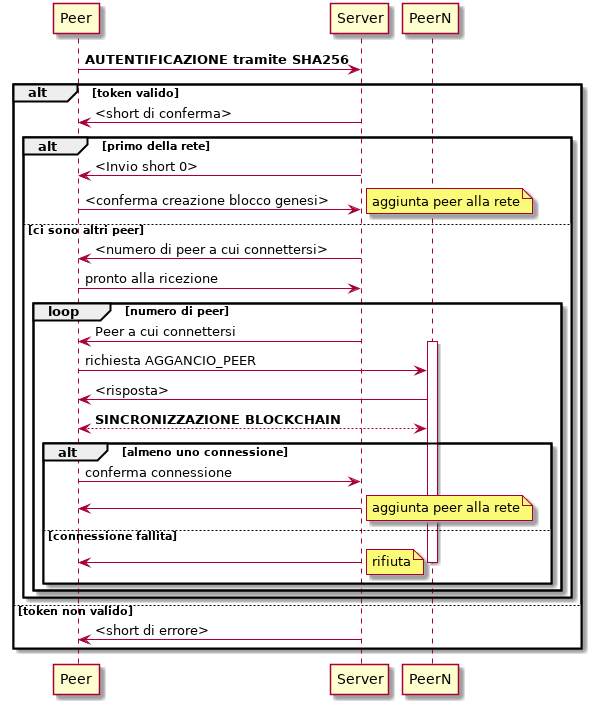
\includegraphics[scale=0.40]{hookpeer.png}
  \caption{Aggancio nodo.}
  \end{figure}
	\newpage
  \section{Aggancio wallet.}
  La procedura dell'aggancio del wallet è più semplice in quanto il wallet invierà al nodo scelto una richiesta del tipo \textbf{request\_t} e in caso di disponibilità il nodo invierà un intero a conferma di avvenuta connessione.

  \begin{figure}[H]
  \center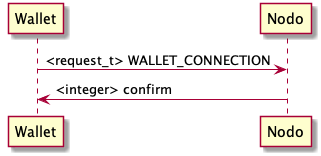
\includegraphics[scale=0.40]{hookwallet.png}
  \caption{Aggancio wallet.}
  \end{figure}

	\section{Invio transazione}
	Dopo aver opportunamente creato una transazione, il wallet provvederà a mandarla al peer a cui è connesso. A seguito di una conferma, il nodo, aggiungerà alla blockchain il blocco appena creato contentente la transazione e provvederà ad inviare a tutti i peer della rete a cui è connesso il blocco.

	\begin{figure}[H]
	\center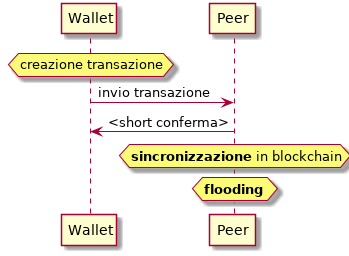
\includegraphics[scale=0.40]{newtransaction.png}
	\caption{Invio transazione.}
	\end{figure}


  \chapter{Dettagli implementativi}
	Per la realizazione di ogni applicativo si è optato per protocolli TCP/IP e Socket di Berkley.
    \section{Dettagli del nodo}\noindent
	I nodi poiché devono spedire i vari blocchi, controllare l'arrivo di nuovi, servire le richieste di connessione e di transazione dei wallet, sono stati implementati secondo uno schema \textbf{I/O Multiplexing} che usa i thread posix della libreria pthread. In particolar modo ad ogni nuova connessione verrà creato un thread che userà a sua volta uno schema I/O Multiplexing. In tal modo un nodo che vuole connettersi ad un peer della rete avrà un thread a gestirgli la connessione, mentre ne avrà \textsc{n} in relazione a quante connessioni avrà ricevuto.\newline
	Per ovviare ai relativi problemi dovuti all’accesso concorrente alla blockchain si è scelto di sincronizzare i thread tramite \textbf{lock rw} disponibili nella libreria \textsc{pthread.h}.

    \section{Dettagli del wallet}\noindent

 I nodi wallet dovendo gestire input da tastiera e l'arrivo dalla rete di richieste dal peer connesso, si è deciso di implementarlo con uno schema I/O Multiplexing come nel caso precedente con la differenza che saranno processi del tutto iterativi, bloccandosi nel caso ci sia attesa dovuta alla connessione.

  \chapter{Manuale utente}
	Il progetto è stato strutturato nel seguente modo: nella cartella src ci saranno i file .c e .h dei due processi sotto opportune cartelle. Nella cartella include vi sono gli header file delle librerie, che si trovano invece nella cartella src. Nella cartella lib viene creata anche la cartella static contentente la libreria statica per il corrispettivo sistema operativo.
	\begin{figure}[H]
  \center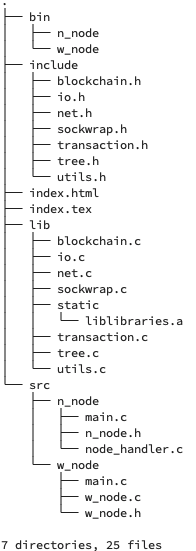
\includegraphics[scale=0.40]{dirs.png}
  \end{figure}




\section{Instruzioni per la compilazione}\noindent	Per la creazione dei file eseguibili si è scelto di affidarsi al software CMake che genera automaticamente il make file.
Per cui basterà creare la cartella build e spostarvici all'interno:
\begin{lstlisting}
$ mkdir build && cd build
\end{lstlisting}
Lanciare cmake con il comando:

\begin{lstlisting}
$ cmake ..
\end{lstlisting}
A seguito della creazione, lanciare make:

\begin{lstlisting}
$ make
\end{lstlisting}
A questo punto nella directory bin saranno presenti i file eseguibili.
\section{Instruzioni per l'esecuzione}\noindent
Per avviare i programmi basterà spostarsi nella cartella bin, e avviare N processi n\_node, e a seguito i processi w\_node. Poiché i processi w\_node si connetteranno alla rete peer to peer tramite opzione da riga di comando andranno eseguiti prima i processi n\_node.
Poiché si presuppone che un ipotetico firewall sia abilitato e che i processi possano essere raggiunti tramite il loro indirizzo pubblico, l'unica opzione attivabile è quella per esporre la porta.
\begin{lstlisting}
$ n_node -p 5555
\end{lstlisting}
I wallet invece possono anche selezionare un indirizzo IP oltre che la porta a cui connettersi. Per motivi pratici è stata aggiunta come opzione facoltativa, per cui:
\begin{lstlisting}
$ w_node -p 5555
\end{lstlisting}
\end{document}
